\let\negmedspace\undefined
\let\negthickspace\undefined
\documentclass[journal]{IEEEtran}
\usepackage[a5paper, margin=10mm, onecolumn]{geometry}
%\usepackage{lmodern} % Ensure lmodern is loaded for pdflatex
\usepackage{tfrupee} % Include tfrupee package

\setlength{\headheight}{1cm} % Set the height of the header box
\setlength{\headsep}{0mm}     % Set the distance between the header box and the top of the text
\usepackage{multicol}
\usepackage{gvv-book}
\usepackage{gvv}
\usepackage{cite}
\usepackage{amsmath,amssymb,amsfonts,amsthm}
\usepackage{algorithmic}
\usepackage{graphicx}
\usepackage{textcomp}
\usepackage{xcolor}
\usepackage{txfonts}
\usepackage{listings}
\usepackage{enumitem}
\usepackage{mathtools}
\usepackage{gensymb}
\usepackage{comment}
\usepackage[breaklinks=true]{hyperref}
\usepackage{tkz-euclide} 
\usepackage{pgfplots}
\pgfplotsset{compat=1.18}
\usepackage{listings}
% \usepackage{gvv}                                        
\def\inputGnumericTable{}                                 
\usepackage[latin1]{inputenc}                                
\usepackage{color}                                            
\usepackage{array}                                            
\usepackage{longtable}                                       
\usepackage{calc}                                             
\usepackage{multirow}                                         
\usepackage{hhline}                                           
\usepackage{ifthen}                                           
\usepackage{lscape}
\usepackage{tikz}
% Marks the beginning of the document
\begin{document}
\bibliographystyle{IEEEtran}
\vspace{3cm}

\title{2007-AE}
\author{EE24BTECH11056 - S.Kavya Anvitha}
\maketitle
%\newpage
\bigskip

\renewcommand{\thefigure}{\theenumi}
\renewcommand{\thetable}{\theenumi}
\begin{enumerate}
\item $\lim_{x \to 0} \frac{\sin(x)}{e^xx} = $
\begin{enumerate}
    \item $10$
    \item $0$
    \item $1$
    \item $\infty$\\
\end{enumerate}
\item Let a dynamical system be described by the differential equation $2\frac{dx}{dt} + \cos{x} = 0$.Which of the following differential equations describes this system in a close approximation sense for small perturbation about $x = \frac{\pi}{4}$
\begin{enumerate}
    \item $2\frac{dx}{dt} + \sin{x} = 0$
    \item $2\frac{dx}{dt} - \frac{1}{\sqrt{2}} = 0$
    \item $\frac{dx}{dt} + \cos{x} = 0$
    \item $\frac{dx}{dt} + x = 0$\\
\end{enumerate}

Common Data for Questions $71, 72 \& 73$: An airplane designer wants to keep longitudinal static stability margin (SM) within $5\% to 15\%$ of mean  aerodynamic chord.A wind tunnel test of the model showed that for $\Bar{X_{\text{CO}_2}} = 0.3$,$\frac{dC_{\text{m}}}{dC_{\text{L}}}$ = $-SM$ holds true for this airplane.\\

\item  The most forward location of the airplane  center of gravity permitted to fulfill the designer's requirement on longitudinal static stability margin is
\begin{enumerate}
    \item $0.35 \Bar{c}$
    \item $0.25 \Bar{c}$
    \item $0.15 \Bar{c}$
    \item $0.52 \Bar{c}$\\
\end{enumerate}
\item The most aft location of the airplane center of gravity permitted to fulfill designer's requirement on longitudinal static stability is
\begin{enumerate}
    \item $0.35 \Bar{c}$
    \item $0.45 \Bar{c}$
    \item $0.52 \Bar{c}$
    \item $0.67 \Bar{c}$\\
\end{enumerate}
\item The center of gravity location to have $\frac{d\delta_{\text{e}}}{dC_{\text{L}}} = 0$ is
\begin{enumerate}
    \item $0.35 \Bar{c}$
    \item $0.45 \Bar{c}$
    \item $0.5 \Bar{c}$
    \item $0.4 \Bar{c}$\\ 
\end{enumerate}
Common Data for Questions $74 \& 75$: Consider the spring mass system shown in figure below. This system mass system shown in figure below. This system has two degrees of freedom representing the motions of the two masses. 


\begin{tikzpicture}

% Drawing masses
\draw[thick] (0,0) rectangle (1.5,-1) node[midway] {$m$};
\draw[thick] (4,0) rectangle (5.5,-1) node[midway] {$3m$};

% Drawing springs
\draw[thick, decorate, decoration={coil, aspect=0.6, segment length=5mm, amplitude=3mm}] 
(-2,0) -- (0,0);
\draw[thick, decorate, decration={coil, aspect=0.6, segment length=5mm, amplitude=3mm}] 
(1.5,0) -- (4,0);
\draw[thick, decorate, decoration={coil, aspect=0.6, segment length=5mm, amplitude=3mm}] 
(5.5,0) -- (7.5,0);

% Labels for springs
\node at (-1, 0.6) {$k$};
\node at (2.75, 0.6) {$k$};
\node at (6.5, 0.6) {$k$};

% Ground representation
\draw[thick] (-2,-1) -- (7.5,-1);

% Labels for positions
\draw[->] (0.75,1) -- (0.75,0);
\node at (0.75,1.4) {$x_1$};

\draw[->] (4.75,1) -- (4.75,0);
\node at (4.75,1.4) {$x_2$};

\end{tikzpicture}

\item The system shows the following type of coordinate coupling
\begin{enumerate}
    \item static coupling
    \item dynamic coupling
    \item static and dynamic coupling
    \item no coupling\\
\end{enumerate}
\item The two natural frequencies of the system are given as
\begin{enumerate}
    \item $\sqrt{\frac{4+\sqrt{5}}{3}\frac{k}{m}}$
    \item $\sqrt{\frac{4+\sqrt{3}}{3}\frac{k}{m}}$
    \item $\sqrt{\frac{4+\sqrt{7}}{3}\frac{k}{m}}$
    \item $\sqrt{\frac{4+\sqrt{11}}{3}\frac{k}{m}}$
\end{enumerate}
Linked Answer Questions: $Q.76$ to $Q.85$ carry two marks each.
\section*{Statement for Linked Answer Questions 76 \& 77:}
For a piston propeller airplane weighing 20000 N, the flight testing at $5$ km pressure altitude in standard atmosphere gave the variation of power required versus true air speed as shown in figure below. The student forgot to label the air speed axis. The maximum climb rate at sea level was calculated to be 4 m/s. Assume shaft power available to be independent of speed of flight. For piston propeller airplane, it can be assumed that the shaft power available is proportional to ambient density. Values of air density at sea level and at 5 km pressure altitude are $1.225 kg/m^3$ and $0.74 kg/m^3$, respectively.



\begin{tikzpicture}
    % Axes
    \draw[->] (0,0) -- (10,0) node[right] {$V$ (True air speed)};
    \draw[->] (0,0) -- (0,6) node[above] {Power Required $P_R$, watts};

    % Power required ticks and labels
    \node at (-0.8,5) {$15 \times 10^4$};
    \node at (-0.8,3.5) {$10 \times 10^4$};
    \node at (-0.8,2) {$5 \times 10^4$};

    % Horizontal grid lines
    \draw[dashed] (-0.1,5) -- (9,5);
    \draw[dashed] (-0.1,3.5) -- (9,3.5);
    \draw[dashed] (-0.1,2) -- (9,2);

    % Solid curve for sea level
    \draw[thick] plot[smooth] coordinates {(0.5,2.5) (1.5,2.0) (3,1.8) (4.5,2.2) (6,3.0) (8,4.2) (9,5)};

    % Dotted curve for 5 km, offset further to the right for better separation
    \draw[dashed, thick] plot[smooth] coordinates {(1,2.5) (2,2.0) (3.5,1.8) (5,2.2) (6.5,3.0) (8.5,4.2) (9.5,5)};

    % Sea level and 5 km labels
    \node at (9.2,4.5) {5 km};
    \node at (6.5,2.7) {Sea level};

    % Axis labels
    \node at (4.5,-0.5) {V (True air speed)};
    \node[rotate=90] at (-1.5,3) {Power Required $P_R$, watts};

\end{tikzpicture}


\item  The maximum rate of climb achievable by this airplane at $5 km$ altitude will be

\begin{enumerate}
    \item $1.65 m/s$
    \item $0.51 m/s$
    \item $1.43 m/s$
    \item $3.65 m/s$\\
\end{enumerate}

\item If during the maximum rate of climb at $5 km$ altitude, the airplane was flying at an angle of attack of $4$ degrees and attitude (pitch) angle of $5$ degrees, what was equivalent airspeed of the airplane?

\begin{enumerate}
    \item  $40.2 m/s$
    \item  $63.7 m/s$
    \item  $130.3 m/s$
    \item  $20.2 m/s$\\
\end{enumerate}

\section*{Statement for Linked Answer Questions $78$ \& $79$:}
A model wing of rectangular planform has a chord of $0.2 m$ and a span of $1.2 m$. It has a symmetric airfoil section whose lift curve slope is $0.1$ per degree. When this wing is mounted at $8$ degrees angle of attack in a freestream of 20 m/s it is found to develop $35.3 N$ lift when the density of air is $1.225 kg/m^3$.\\

\item The lift curve slope of this wing is:
\begin{enumerate}
    \item  $0.10 per deg$
    \item  $0.092 per deg$
    \item  $0.075 per deg$
    \item  $0.050 per deg$\\
\end{enumerate}

\item The span efficiency factor of this wing is:
\begin{enumerate}
    \item  $1.0$
    \item  $0.91$
    \item  $0.75$
    \item  $0.63$\\
\end{enumerate}

\section*{Statement for Linked Answer Questions $80 \& 81$:}
Let $F(s) = \frac{s+10}{(s+2)(s+20)}$\\

\item The partial fraction expansion of $F(s)$ is:
\begin{enumerate}
    \item  $\frac{1}{s+2} + \frac{1}{s+20}$
    \item  $\frac{5}{s+2} + \frac{2}{s+20}$
    \item  $\frac{2}{s+2} + \frac{20}{s+20}$
    \item  $\frac{4/9}{s+2} + \frac{5/9}{s+20}$\\
\end{enumerate}

\item The inverse Laplace transform of $F(s)$ is:
\begin{enumerate}
    \item  $2e^{-2t} + 20e^{-20t}$
    \item  $\frac{4}{9}e^{-2t} + \frac{5}{9}e^{-20t}$
    \item  $5e^{-2t} + 2e^{-20t}$
    \item  $\frac{9}{5}e^{-2t} + \frac{4}{9}e^{-20t}$\\
\end{enumerate}

\section*{Statement for Linked Answer Questions $82 \& 83$:}
The equation of motion of a vibrating rod is given by $\frac{\partial^2 u}{\partial t^2} = c^2 \frac{\partial^2 u}{\partial x^2}$. Here $u$ is the displacement along the rod and is a function of both position $x$ and time $t$. To find the response of the vibrating rod, we need to solve this equation using boundary conditions and initial conditions.\\

\item The boundary conditions needed for a rod fixed at the root ($x = 0$) and free at the tip ($x = l$) are:
\begin{enumerate}
    \item  $u(x=0) = 0, \frac{\partial u}{\partial x}(x = l) = 0$
    \item  $u(x=l) = 0, \frac{\partial u}{\partial x}(x = l) = 0$
    \item  $u(x=0) = 0, u(x=l) = 0$
    \item  $\frac{\partial u}{\partial x}(x=0) = 0, \frac{\partial u}{\partial x}(x=l) = 0$\\
\end{enumerate}

\item The natural frequencies $\omega$ of the fixed-free rod can then be obtained using:
\begin{enumerate}
    \item  $\cos \brak{\frac{\omega l}{c}} = 0$
    \item  $\sin \brak{ \frac{\omega l}{c}} = 0$
    \item  $\cosh \brak{ \frac{\omega l}{c}} = 0$
    \item  $\cos \brak{\frac{\omega l}{c}} = 0$\\
\end{enumerate}

\section*{Statement for Linked Answer Questions $84 \& 85$:}
Air enters the compressor of a gas turbine engine with velocity $127 m/s$, density $1.2 kg/m^3$ and stagnation pressure $0.9 MPa$. Air exits the compressor with velocity $139 m/s$ and stagnation pressure $3.15 MPa$. Assume that the ratio of specific heats is constant and equal to $1.4$.\\

\item The compressor pressure ratio is:
\begin{enumerate}
    \item  $0.22$
    \item  $0.28$
    \item  $3.50$
    \item  $3.90$\\
\end{enumerate}

\item If the polytropic efficiency of the compressor is $0.89$, then the isentropic efficiency of the compressor is:
\begin{enumerate}
    \item  $0.613$
    \item  $0.869$
    \item  $0.89$
    \item  $0.98$\\
\end{enumerate}

\end{enumerate}
\end{document}
o
